\documentclass[tikz,border=2pt]{standalone}
\usepackage{amsmath}
\usepackage{pgfplots}
\pgfplotsset{compat=1.18}

\begin{document}
% a_n = (-1)^n (1 + 2/n): the tails' suprema decrease to limsup = 1, the tails' infima increase
% to liminf = -1; the sequence itself has no limit.
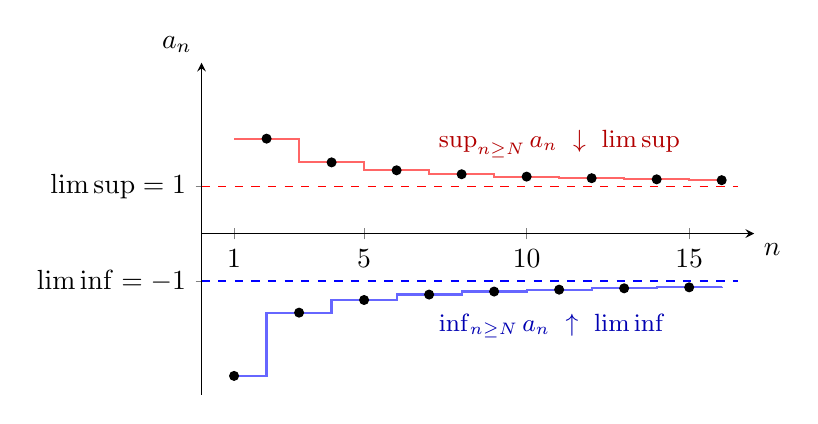
\begin{tikzpicture}
	\begin{axis}[
		axis lines=middle,
		xmin=0, xmax=17,
		ymin=-3.4, ymax=3.6,
		xtick={1,5,10,15}, ytick={-1,1}, yticklabels={$\liminf=-1$,$\limsup=1$},
		xlabel={$n$}, ylabel={$a_n$},
		xlabel style={below right}, ylabel style={above left},
		clip=false,
		width=8.6cm, height=5.8cm
		]
		\addplot[red, dashed, domain=0:16.5] {1};
		\addplot[blue, dashed, domain=0:16.5] {-1};
		% sup of tails: 1+2/n at even n (step function), inf of tails: -(1+2/n) at odd n
		\addplot[red!60, thick, const plot, no marks] coordinates {(1,2) (2,2) (3,1.5) (4,1.5) (5,1.333) (6,1.333) (7,1.25) (8,1.25) (9,1.2) (10,1.2) (11,1.167) (12,1.167) (13,1.143) (14,1.143) (15,1.125) (16,1.125)};
		\addplot[blue!60, thick, const plot, no marks] coordinates {(1,-3) (2,-1.667) (3,-1.667) (4,-1.4) (5,-1.4) (6,-1.286) (7,-1.286) (8,-1.222) (9,-1.222) (10,-1.182) (11,-1.182) (12,-1.154) (13,-1.154) (14,-1.133) (15,-1.133) (16,-1.125)};
		\addplot[only marks, mark=*, mark size=1.6pt, black, samples at={1,...,16}] {(-1)^x*(1+2/x)};
		\node[red!70!black, anchor=south west, font=\small] at (axis cs:7,1.4) {$\sup_{n\ge N}a_n\ \downarrow\ \limsup$};
		\node[blue!70!black, anchor=north west, font=\small] at (axis cs:7,-1.5) {$\inf_{n\ge N}a_n\ \uparrow\ \liminf$};
	\end{axis}
\end{tikzpicture}
\end{document}
